\documentclass[9pt]{pnas-new}
\RequirePackage[slovene,english]{babel} % when writing in english
\templatetype{pnasresearcharticle} % Choose template 
\selectlanguage{english}


\usepackage{graphicx}
\usepackage{subfig}
% \usepackage[dvipsnames]{xcolor}
% \usepackage[usenames,dvipsnames]{color}

\usepackage{hyperref}
\hypersetup{colorlinks=true, linkcolor=blue, linktocpage}

\usepackage{import}
\usepackage[subpreambles=true]{standalone}


\definecolor{amber}{rgb}{1.0, 0.49, 0.0}
\definecolor{cadmiumorange}{rgb}{0.93, 0.53, 0.18}
\definecolor{carrotorange}{rgb}{0.93, 0.57, 0.13}

% Fancy new commands
\newcommand{\set}[1]{\ensuremath{\mathbf{#1}}}
\renewcommand{\vec}[1]{\ensuremath{\mathbf{#1}}}
\newcommand{\uvec}[1]{\ensuremath{\hat{\vec{#1}}}}
\newcommand{\const}[1]{{\ensuremath{\kappa_\mathrm{#1}}}} 
\newcommand{\num}[1]{#1}

% Path settings
\graphicspath{{./figures/}}





















\title{Simulating flock of birds using only vision}

\author{Žiga Leskovec}
\author{Maksimiljan Vojvoda}
\affil{Collective behaviour course research seminar report} 
\leadauthor{Leskovec \& Vojvoda} 

\selectlanguage{english}

\significancestatement
{A model of collective behavior based purely on vision}
{
When modeling collective behaviour it is commonly assumed that agents inherently know other agents position, velocity and direction.
There exists a motivation to get rid of these assumptions and model the behaviour based on how internal and external information is acquired and processed.
Vision is one of the more important sensory systems that provide crucial external information, which turns out to be sufficient for modeling interactions between agents in a swarm.
In this seminar we explore a mathematical framework for perception-based interactions proposed by Renaud Bastien and Pawel Romanczuk.
}
{Simulation | Vision | Flock of birds }


% Please include corresponding author, author contribution and author declaration information
% \authorcontributions{Please provide details of author contributions here.}
%\authordeclaration{Please declare any conflict of interest here.}
%\equalauthors{\textsuperscript{1}A.O.(Author One) and A.T. (Author Two) contributed equally to this work (remove if not applicable).}
%\correspondingauthor{\textsuperscript{2}To whom correspondence should be addressed. E-mail: author.two\@email.com}

% Keywords are not mandatory, but authors are strongly encouraged to provide them. If provided, please include two to five keywords, separated by the pipe symbol, e.g:
\keywords{Simulation | Vision | Flock of birds }
\begin{abstract}
When modeling collective behaviour it is commonly assumed that agents inherently know other agents position, velocity and direction.
There exists a motivation to get rid of these assumptions and model the behaviour based on how internal and external information is acquired and processed.
Vision is one of the most important sensory systems that provide crucial external information, which turns out to be sufficient for modeling interactions between agents in a swarm.
In this seminar we explore a mathematical framework for perception-based interactions proposed by Renaud Bastien and Pawel Romanczuk.
\end{abstract}

\dates{\textbf{\today}}
\program{BM-RI}
\vol{2023/24}
\no{CB:F} % group ID
%\fraca{FRIteza/201516.130}

\begin{document}

% Optional adjustment to line up main text (after abstract) of first page with line numbers, when using both lineno and twocolumn options.
% You should only change this length when you've finalised the article contents.
\verticaladjustment{-2pt}

\maketitle
\thispagestyle{firststyle}
\ifthenelse{\boolean{shortarticle}}{\ifthenelse{\boolean{singlecolumn}}{\abscontentformatted}{\abscontent}}{}

\dropcap{M}odels of collective behaviour often rely on interactions that do not have a direct physical reality (such as neighbour velocity, relative position and direction).
One example of this is the simulation of fish schools \cite{wissel1992fish}.
However, this assumption of how the information is processed by agents limits our understanding of the underlying complexity that takes place in such phenomena.
A better alternative would be to model the behaviour around internal and external information that agents are capable of acquiring.

In this seminar we use a mathematical framework proposed by Renaud Bastien and Pawel Romanczuk \cite{main-paper}, to create a simulation of flock of birds that solely relies on vision.
We improve on the original paper by replacing ray casting with direct projection, which increases accuracy and computational speed of each simulation step.
Finally, we also introduce colors to the visual field projections, which in turn allow us to model more versatile collective behaviours with different agent types (e.g. predator, prey, disruptor ...).


% <---- look at it, litle fella right there
% huh?























\section*{Methods}

The simulation is done in 2-dimensional space where agents are represented as simple disk objects with full $360^\circ$ view.
On each simulation step, their velocity is modified based on a projection of their surrounding visual field.

The parameters that encode the severity of the response to the environment can also be upgraded with the use of \textit{colors}, where parameters vary between each color.
In other words, a boid can have different responses to different kinds of objects in their surroundings.

This simulates a primitive form of vision.





\subsection{Visual field projection}

\begin{figure}
    \centering
    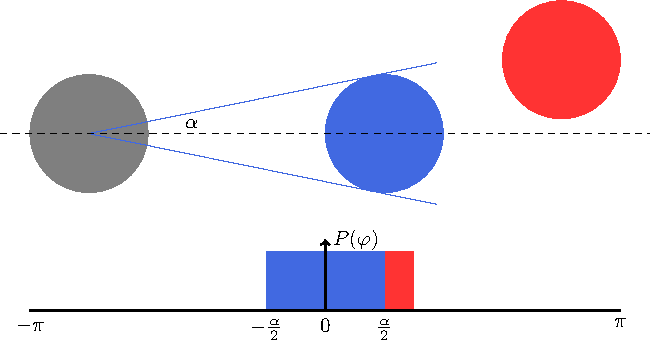
\includegraphics[width=0.7\linewidth]{figures/projection-colored.pdf}
    \caption{
       Projection field graph of an object. The projection interval of the blue object overlaps (overrides) part of the interval of the red object.
    }
    \label{fig:example-projection}
\end{figure}

\sloppy

Objects around the agent are projected onto their visual field, described by $P(\varphi)$.
Function $P(\varphi)$ represents visual obstructions of the agent, where $\varphi$ is an angle of the visual field. The result is binary, where 0 represents ``not obstructed'' and 1 represents ``obstructed''.
An example of a visual field projection can be seen on figure \ref{fig:example-projection}.

\fussy


\subsection{Colored visual projection field}

After achieving the basic monochrome visual projection field, we can extend it to also hold information about the color of the projected object as shown on figure \ref{fig:example-projection}.
This will come in handy when implementing different behavioral responses to different surrounding objects.
This allows us to implement \textit{disruptor} birds to make the simulation a bit more interesting.

We must be careful to ensure that projection intervals of closer objects take precedent over more distant objects.
In other words, we must sort objects based on distance just like in regular computer graphics.
Just like in computer graphics, we don't actually sort the objects, we instead keep a z-index (or depth index) of each projection interval and then override intervals with larger z-indexes.





\subsection{Velocity}

On each simulation step, the velocity of agent $i$, is modified by $\Delta v_i$.
The general speed delta is summarized with the following equation:

\begin{equation}
    \Delta v_i = \text{F}_{\text{ind}}(v_i) + \text{F}_{\text{vis}}(P_i)
\end{equation}

where $\text{F}_{\text{ind}}$ function represents speed delta collected from \textbf{ind}ividuals ``internal information'':

\begin{equation}
    \text{F}_{\text{ind}} = \gamma(v_\text{pref} - v_i)\hat{v_i}
\end{equation}

where $\gamma$ represents speed relaxation rate, $v_\text{pref}$ \textbf{pref}erred speed of the individual and $\hat{v_i}$ normalized direction vector.
Function $\text{F}_{\text{vis}}$ transforms \textbf{vis}ual field to the individuals speed delta.
It is independent of other individuals properties, and is described with the following equation:

\begin{equation}
    \text{F}_{\text{vis}}(P) = \int_{-\pi}^{\pi} \ G(P, \varphi) \ h(\varphi) \ d\varphi
\end{equation}

Here $G(P, \varphi)$ encodes how information from the visual field impacts the movement, while $h(\varphi)$ encodes properties of the perception-motor system, in our case, it describes how front-back distance impacts the speed and how left-right distance influences the heading direction of an agent.
For convenience the equation is split into two parts
\sloppy

\begin{equation}
    \Delta v_i = \gamma(v_\text{pref} - v_i) +
        \int_{-\pi}^{\pi} cos(\varphi) \ \alpha_0
        \left(
            -P_i(\varphi) \ + \ \alpha_1 (\partial_{\varphi} P_i(\varphi))^2
        \right) d\varphi
    \label{eq:speed}
\end{equation}


\begin{equation}
    \Delta \Psi_i =
        \int_{-\pi}^{\pi}
        sin(\varphi) \ \beta_0
        \left(
            -P_i(\varphi) \ + \ \beta_1 (\partial_{\varphi} P_i(\varphi))^2
        \right) d\varphi
    \label{eq:angle}
\end{equation}

The first ($\Delta v_i$) describes speed delta, while the second ($\Delta \Psi_i$) describes heading angle delta.
Consequently the heading vector is now removed, since it is encoded as the heading angle.

As we will see further in the seminar, parameters $\alpha_1$ and $\beta_1$ influence the equilibrium distances.
$\alpha_1$ influences the front-back distance equilibrium $\frac{r}{\alpha_1}$, while $\beta_1$ influences the left-right distance equilibrium $\frac{r}{\beta_1}$, where $r$ stands for agent radius.

For a more realistic simulation we also added parameter $v_{\textbf{max}}$ that constraints boid's speed.
This was needed when adding \textit{disruptor} boids, as their repulsive/attractive behaviour resulted in unrealistic speeds (compared to $v_{\text{pref}}$)




\subsection{Integration of P}

One of the core elements of the simulation is calculating integrals of functions multiplied with $P$ such as $\int_{-\pi}^{\pi} cos(\varphi) P_i(\varphi)$ from equations \ref{eq:angle} and \ref{eq:speed}.
Because the projection function $P$ contains contiguous regions of values $0$ or $1$, we can split the integral into multiple definite integrals where we calculate only the sections where $P$ has value of $1$.
A visual representation of multiplying a trigonometric function with $P$ (in this case $cos$) can be seen on figure \ref{fig:integral}.
This trick trivialises the integral calculation.

With colored projection fields, we must also take into consideration that each interval has a different set of constants ($\alpha_0$, $\alpha_1$, $\beta_0$, ...).
This doesn't change much as all we must do is retrieve the appropriate constants of the \textit{colored} interval we are currently handling.


\begin{figure}[h]
    \centering
    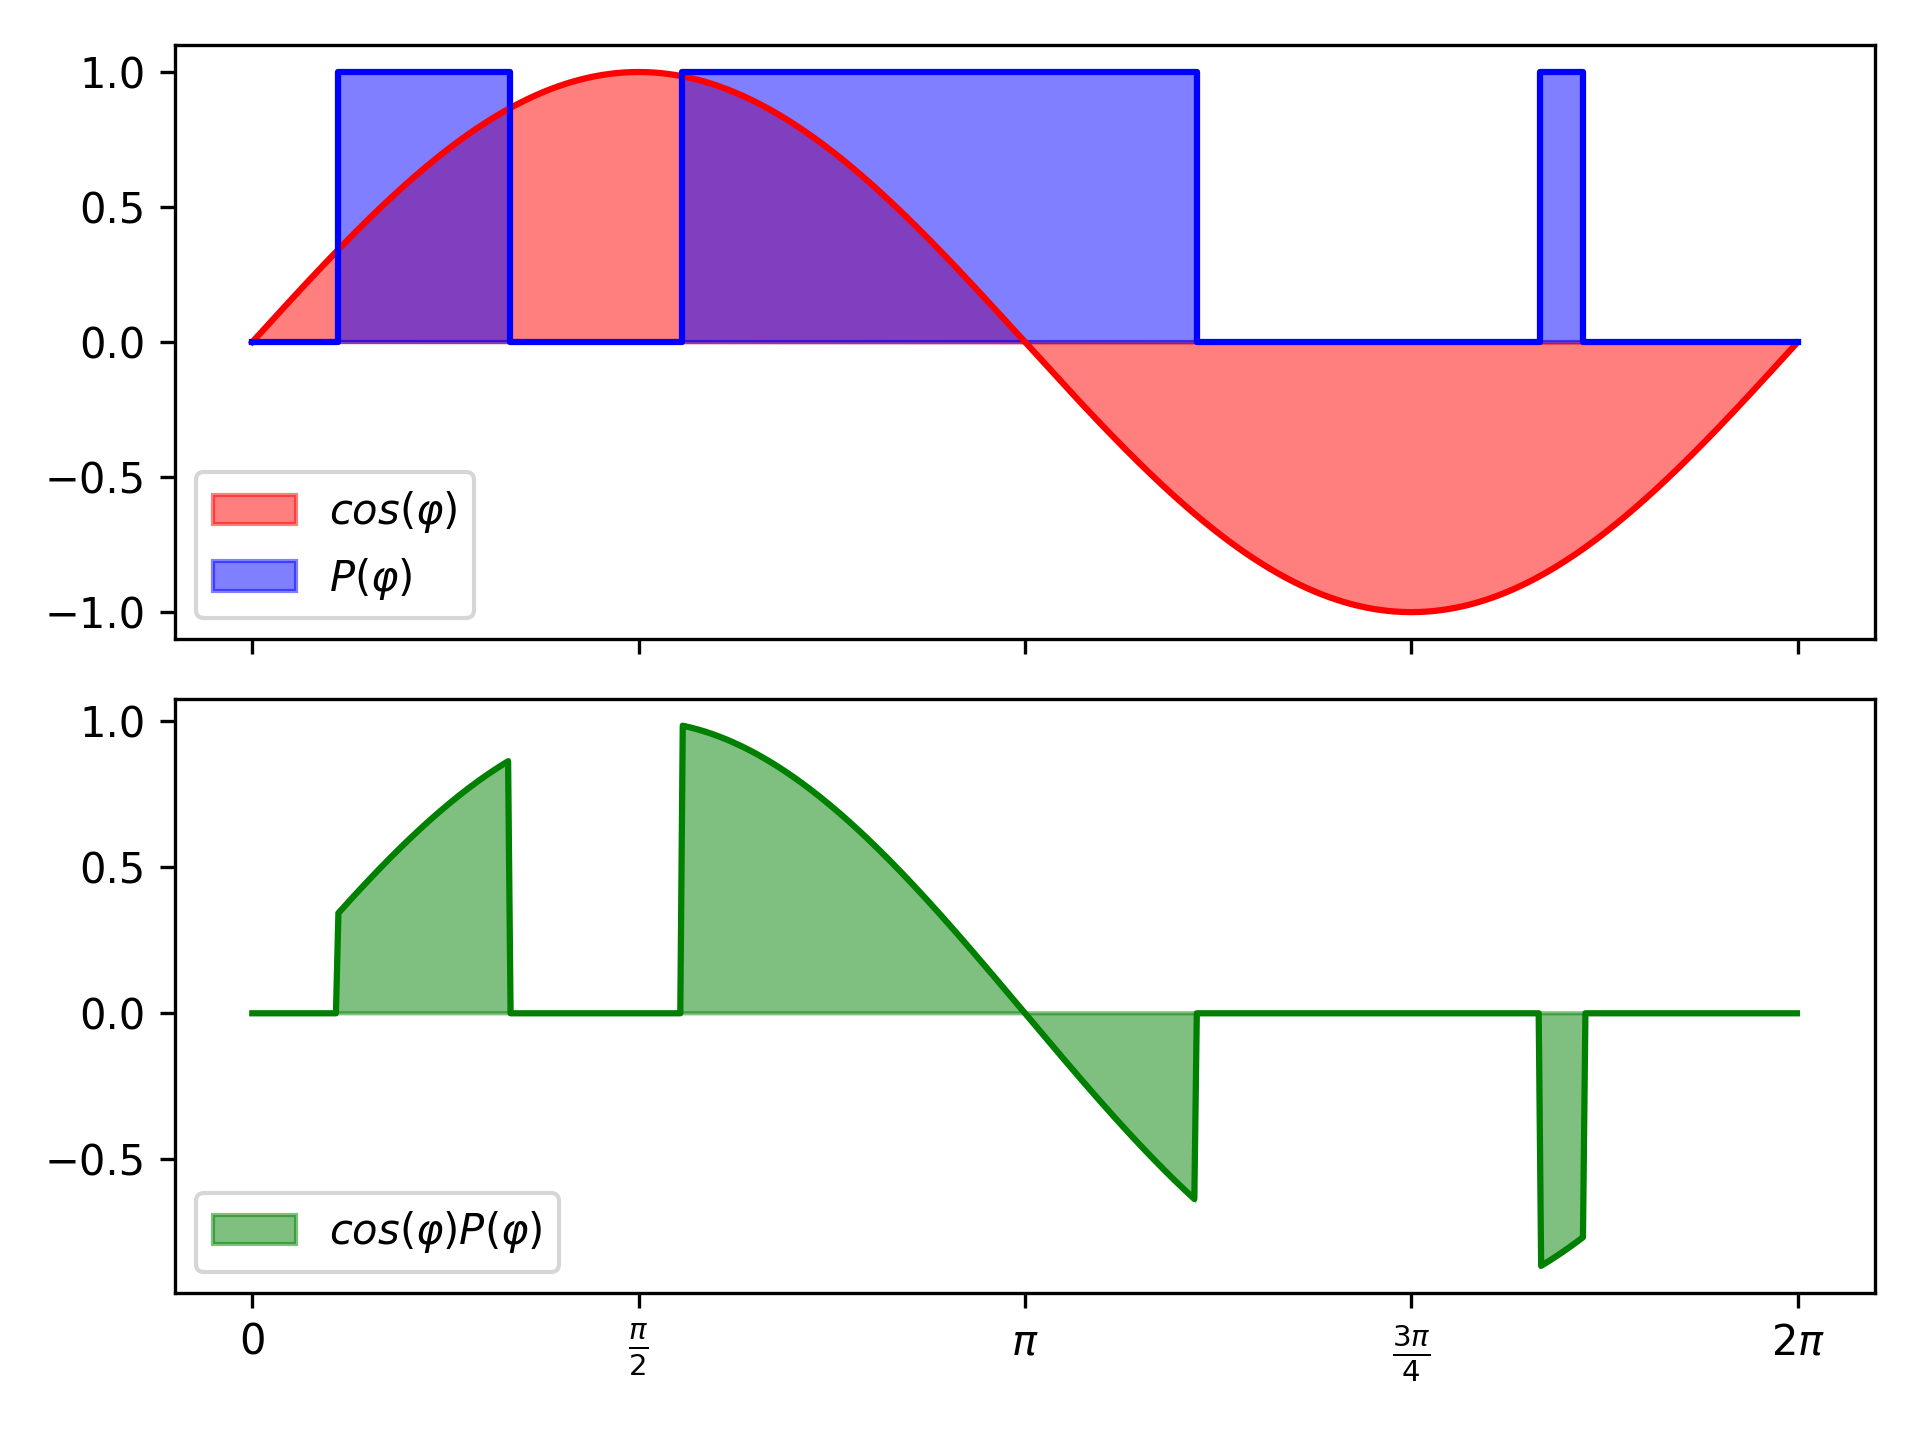
\includegraphics[width=0.6\linewidth]{integral.png}
    \caption{
      Multiplying a function (in this case $cos$) with some projection function $P$.
    }
    \label{fig:integral}
\end{figure}




\subsection{Implementation}

The simulation is implemented in C++.

In the source paper \cite{main-paper}, the author calculates the projection function $P$ using ray casting.
Ray casting is a method of sampling the environment for obstructions by calculating intersections of \underline{all} objects with a line (a ray).
Casting more rays results in a more accurate sampling of the environment.
This is also highly inefficient, as one would have to cast an enormous amount of rays to gain a very precise insight into their environment.

We have improved on this by projecting the objects directly by calculating the appropriate angles of vision for each object as show in figure \ref{fig:example-projection}.
For each object we constructed an array of intervals where $P$ would have a value of $1$.
By carefully merging these intervals we kept the array \textit{clean} as none of the intervals would intersect.
With this array we could trivially calculate all the necessary components described in equations \ref{eq:speed} and \ref{eq:angle} using the method described in the previous section.


The underlying simulation loop is also parallelizable, as agents are dependant only on the previous state of the simulation, therefore we can use multi-threading to increase the simulation speed, thus allowing us to simulate larger or longer simulations.







\subsection{Simulation visualisation}

% Visualisation of the simulation will be done using FFmpeg\footnote{\url{https://ffmpeg.org/}}, which will encode an array of pixels (representing a state of the simulation) into an image or a video.
The speed of image generation is not important to this seminar and is therefore done separately in Python with Matplotlib.
Every simulation figure has its own one minute long animation available on our Github repository \url{https://github.com/siggsy/collective-vision/tree/main/results}.
It is worth noting that the size of the agents is not to scale.


\section*{Results}

Every simulation was run for 2000 steps with 50 agents randomly placed in a box bounded by $(0,0)$ and $(5,5)$.
All agents had a radius of $0.5$ and had $v_\text{pref}$ set to $0.5$.
Simulation parameters were set to the following values:
\begin{enumerate}[label=$\bullet$]
    \item $\alpha_1 = 0.08$
    \item $\beta_1 = 0.08$
    \item $\gamma = 0.95$
\end{enumerate}

In figure \ref{fig:simulation} we can see 3 different collective behaviours using $\alpha_0$ and $\beta_0$ parameters found in the paper this seminar is based on\cite{main-paper}.

\begin{figure}[H]
    \centering
    \begin{tabular}{cc}
        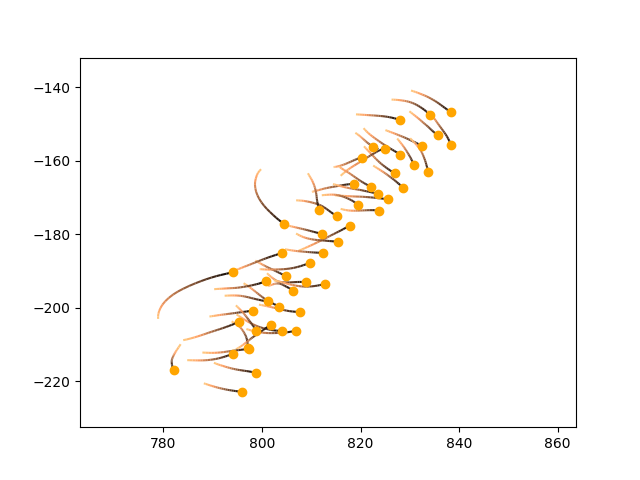
\includegraphics[width=0.466\textwidth]{line.png} &
        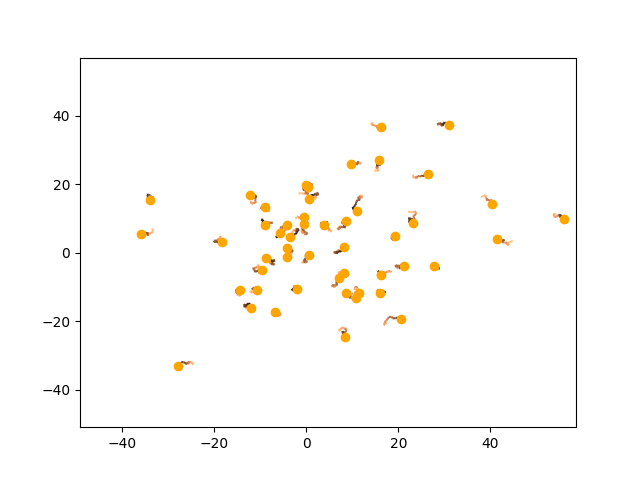
\includegraphics[width=0.466\textwidth]{crystal.png} \\
        (a) Polarized line ($\alpha_0 = 0.5$, $\beta_0 = 0.01$) & (b) Crystal ($\alpha_0 = 0.1$, $\beta_0 = 10$) \\
        \multicolumn{2}{c}{
            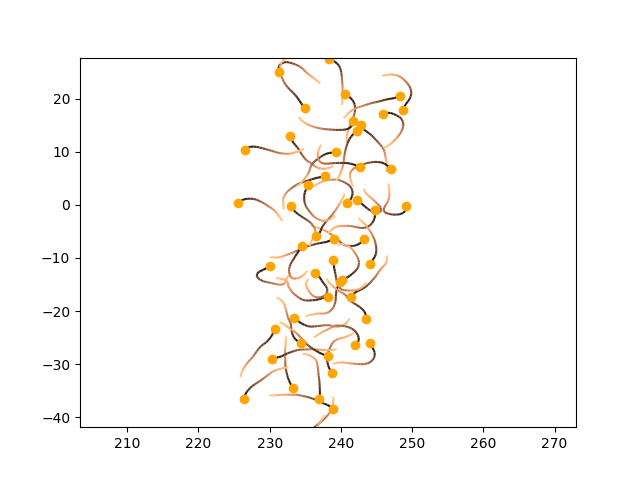
\includegraphics[width=0.5\textwidth]{swarm.png}
        } \\
        \multicolumn{2}{c}{(c) Swarm ($\alpha_0 = 0.5$, $\beta_0 = 1$)}
    \end{tabular}
    \caption{Last frames of the tested simulations}
    \label{fig:simulation}
\end{figure}

In simulation (a) all agents move in one general direction and form a line.
In contrast, in simulation (b) agents shake in-place and barely make any distance.
Since the figures represent the last frames of the animation, this can be observed by checking their final coordinates.
In the final simulation (c) agents are moving around freely while maintaining a swarm.

When observing these behaviours, we can intuitively understand parameter $\alpha_0$ as boid's drive to maintain equilibrium distance by changing its speed, and parameter $\beta_0$ as boid's drive to maintain equilibrium distance by changing its heading direction.

\medskip

Next we tried a simulation with one \textit{disruptor boid (\textcolor{blue}{\textbf{blue}})}.
The parameters for \textcolor{orange}{\textbf{orange}} boids were similar to the ones for a polarized line ($\alpha_0 = 0.5$, $\beta_0 = 0.08$).
The new blue boid has a strong attraction to the orange boids and has higher maximum velocity.
On the other hand, the orange boids strongly avoid the blue boid.

A few frames of the simulation can be seen on figure \ref{fig:simulation-multicolored}, where each frame also shows a graph of the projection field of the outlined orange boid.
In frame (a), the orange boids have not yet encountered the blue boid and continue towards the right.
In frame (b) they finally meet and turn around to try to fly away.
In frame (c) the blue boid finally catches up to the other boids and disperses them.
Frame (d) shows the general chaos of the whole flock as the blue boid franticly tries to catch an orange boid.


\begin{figure}[H]
    \centering
    \begin{tabular}{cc}
        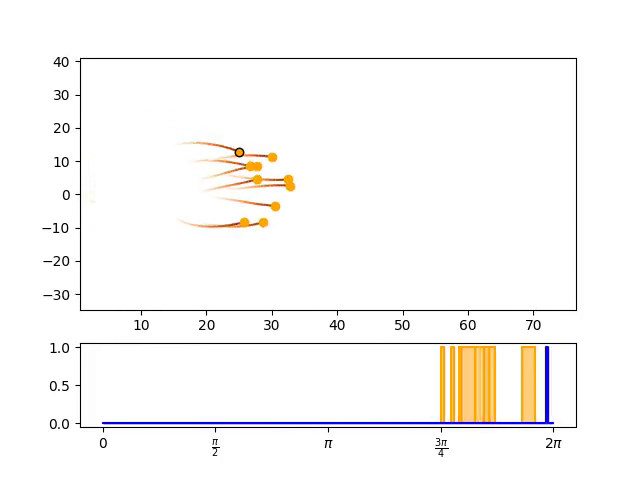
\includegraphics[width=0.47\textwidth]{56.png} &
        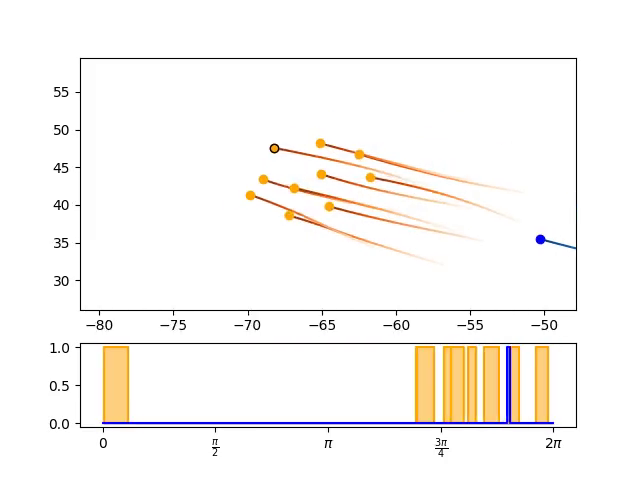
\includegraphics[width=0.47\textwidth]{470.png} \\
        (a) Frame 56. & (b) Frame 470. \\
        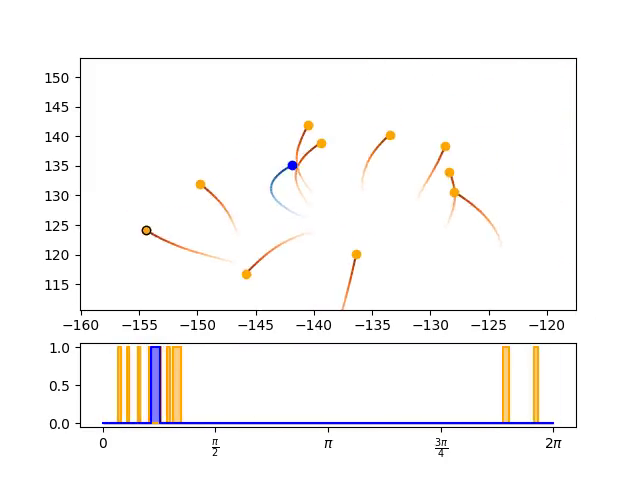
\includegraphics[width=0.47\textwidth]{695.png} &
        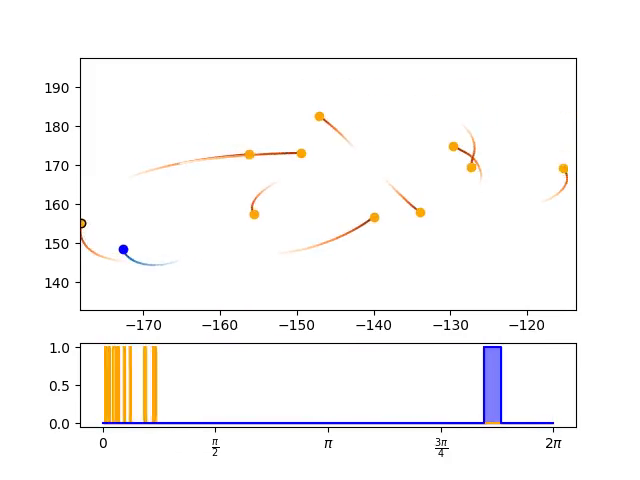
\includegraphics[width=0.47\textwidth]{912.png} \\
        (c) Frame 695. & (d) Frame 912. \\
    \end{tabular}
    \caption{A simulation with an added graph of a projection field of one boid.}
    \label{fig:simulation-multicolored}
\end{figure}























\section*{Discussion}


In this seminar we successfully implemented and reproduced different collective behaviours of birds using only their vision as described in the original work by Bastien and Romanczuk \cite{main-paper}.
The implementation was improved by replacing ray casting with direct projection.
This increased the accuracy and calculation efficiency of the visual fields of the birds.

We have also implemented the \textit{color} information of each projection interval as that allowed us to implement different kinds of boids (regular boids and disruptor/predator boids), as originally proposed in the paper but not implemented.

The simulation is limited to only 2 dimensions as visualisation of more would be quite cumbersome. 

The whole project is available on our GitHub repository \url{https://github.com/siggsy/collective-vision}.

% OLD
% In this seminar we implemented and simulated a collective behaviour of birds using only their vision.

% We have improved on the original work by Bastien and Romanczuk \cite{main-paper} by replacing ray casting with direct projection.
% This improved the accuracy and calculation efficiency of the visual fields of the birds.

% We have also implemented the \textit{color} information of each projection interval as that allowed us to implement different kinds of boids (regular boids and disruptor/predator boids), as originally proposed in the paper but not implemented.

% The simulation is limited to only 2 dimensions as visualisation of more would be quite cumbersome. 

% The whole project is available on our GitHub repository \url{https://github.com/siggsy/collective-vision}.


















\acknow{Žiga Leskovec fine tuned the simulation parameters and handled the simulation visualisation; Maksimiljan Vojvoda implemented the simulation loop.}
\showacknow % Display the acknowledgments section

% \pnasbreak splits and balances the columns before the references.
% If you see unexpected formatting errors, try commenting out this line
% as it can run into problems with floats and footnotes on the final page.
%\pnasbreak

\begin{multicols}{2}
\section*{\bibname}
% Bibliography
\bibliography{./bibliography}
\end{multicols}

\end{document}